\newcommand*{\ddt}[1]{\frac{\partial #1}{\partial t}}

\introsection{Уравнения Максвелла в веществе}

Начало современной, классической, макроскопической электродинамики сплошных сред было положено открытием двух
экспериментальных законов: в 1820 году Ампер установил закон взаимодействия электрических токов. Одной из формулировок
этого закона является теорема о циркуляции вектора напряжённости магнитного поля $\vec{H}$:
\[
\oint_{\Gamma}\vec{H}\,d\vec{l}=I,
\]
где $I$~--- полный ток через замкнутый контур $\Gamma$, а в 1831~году Фарадей экспериментально открыл и сформулировал
явление электромагнитной индукции:
\[
\oint_{\Gamma}\vec{E}\,d\vec{l}=-\frac{d}{dt}\int_S\vec{B}\, d\vec{S}.
\]
Максвелл постулировал, что эти законы имеют силу совершенно независимо от присутствия в пространстве проводящих пробных
контуров, т.~е. магнитное поле и вихревое электрическое поле являются объективной реальностью. Этот постулат лежит в
основе теории электромагнитного поля, а вытекающие из него уравнения Максвелла~--- фундамент современной электродинамики
сплошных сред. В системе СИ эти уравнения имеют следующий вид:

%TODO: уравнения Максвелла

%\def\mmlskip{\vskip 0.5ex plus 0.2ex minus 0.1ex}
%\def\mmlI{\kern10mm}
%\def\mmlII{\kern50mm}
%\def\mml#1#2#3{\par
%\mmlskip
%\noindent\mmlI\hbox to 0pt{$\displaystyle #1$\hss}\mmlII\hbox{$\displaystyle #2$}\hfill\hbox{$#3$}%
%\mmlskip
%}
%\mmlskip
%\mml{\text{дифференциальная форма}}{\text{интегральная форма}}{} \mml{\Div\vec{D}=\rho,}{\oint\vec{D}\,d\vec{S}=q,}{\num{1}}
%\mml{\Rot\vec{E}=-\ddt{\vec{B}},}{\oint\vec{E}\,d\vec{l}=-\int\ddt{\vec{B}}\,d\vec{S},}{\num{2}}
%\mml{\Div\vec{B}=0,}{\oint\vec{B}\,d\vec{S}=0,}{\num{3}}
%\mml{\Rot\vec{H}=\vec{j}+\ddt{\vec{D}},}{\oint\vec{H}\,d\vec{l}=\int\vec{j}\,d\vec{S}+\int\ddt{\vec{D}}\,d\vec{S}.}{\num{4}}
%\mmlskip

Уравнение \eqref{1}~--- это одна из форм записи закона Кулона. Уравнение \eqref{2}~--- формулировка закона
электромагнитной индукции Фарадея: изменяющееся во времени магнитное поле порождает вихревое электрическое поле.
Уравнение \eqref{3} утверждает факт отсутствия магнитных зарядов, и, наконец, уравнение \eqref{4} показывает, что магнитное поле
порождается не только движущимися зарядами (первый член в правой части уравнения), но и изменяющимся во времени
электрическим полем. Этот член был введён Максвеллом. Величина $\ddt{\vec{D}}$ по аналогии с $\vec{j}$ называется плотностью
токов смещения.

Фигурирующие в уравнениях \eqref{1}~--~\eqref{4} векторы $\vec{D}$ (электрическая индукция) и $\vec{E}$ (напряжённость электрического
поля), $\vec{B}$ (магнитная индукция) и $\vec{H}$ (напряжённость магнитного поля), $\vec{j}$ и $\vec{E}$ попарно связаны между собой.
Эта связь определяется средой, в которой происходит электромагнитный процесс. Если можно пренебречь электрическими и
магнитными потерями в среде, то уравнения, описывающие связь этих векторов (материальные уравнения), будут иметь вид
\begin{equation} \eqmark{5}
\vec{D}=\varepsilon_0\varepsilon\vec{E},
\end{equation}
\begin{equation} \eqmark{6}
\vec{B}=\mu_0\mu\vec{H},
\end{equation}
\begin{equation} \eqmark{7}
\vec{j}=\lambda\vec{E},
\end{equation}
где $\varepsilon_0$ и $\mu_0$~--- электрическая и магнитная постоянные вакуума, а $\varepsilon$ и $\mu$~--- электрическая и магнитная
проницаемости среды. Характерная для электродинамики величина
\[
c=\frac{1}{\sqrt{\varepsilon_0\mu_0}}
\]
имеет размерность скорости и называется электродинамической постоянной, а численно она равна скорости света в вакууме.


\introsection{Квазистационарное приближение}

\labsection{Электромагнитные волны в проводящей среде} 
В проводящей среде из-за высокой проводимости можно считать, что токи
смещения равны нулю, а основную роль играет ток проводимости. Будем полагать, что объёмные свободные заряды отсутствуют
по всему объёму проводника. Поскольку током смещения мы пренебрегаем, то $\ddt{\vec{D}}=0$, а $\vec{j}=\lambda\vec{E}$, то уравнение
\eqref{4} приобретает вид
\[
\Rot\vec{H}=\lambda\vec{E}.
\]
Продифференцируем это уравнение по времени:
\begin{equation} \eqmark{8}
\Rot\ddt{\vec{H}}=\lambda\ddt{\vec{E}}.
\end{equation}
Уравнение \eqref{2} с учётом материального уравнения \eqref{6} запишется в виде
\[
\Rot\vec{E}=-\mu_0\mu\ddt{\vec{H}}.
\]
Возьмём от обеих частей этого уравнения $\Rot$:
\begin{equation} \eqmark{9}
\Rot\Rot\vec{E}=-\mu_0\mu\Rot\ddt{\vec{H}}.
\end{equation}
Из векторного анализа известно, что
\begin{equation} \eqmark{10}
\Rot\Rot\vec{E}=\Grad\Div\vec{E}-\Delta\vec{E}.
\end{equation}
Подставляя \eqref{10} в \eqref{9} и учитывая, что $\Div\vec{E}=0$, получим
\begin{equation} \eqmark{11}
\Delta\vec{E}=\mu_0\mu\Rot\ddt{\vec{H}}.
\end{equation}
Исключая из уравнений \eqref{8} и \eqref{11} $\Rot\ddt{\vec{H}}$, получим
\begin{equation} \eqmark{12}
\Delta\vec{E}=\mu_0\mu\lambda\ddt{\vec{E}}.
\end{equation}
Совершенно аналогично взяв $\Rot$ от обеих частей уравнения \eqref{4}, а затем сравнив полученное уравнение с уравнением
\eqref{2}, найдём, что
\begin{equation} \eqmark{13}
\Delta\vec{H}=\mu_0\mu\lambda\ddt{\vec{H}}.
\end{equation}

%TODO: figure

%\rfr[11]{30mm}{1}{}{1}{
%\psfrag{x}[tr]{$x$}
%\psfrag{z}{$z$}
%\psfrag{a}[cl]{$E_0e^{i\omega t}$}
%\psfrag{b}[cl]{$E_x(z,\,t)$}
%}


\introsubsection{Скин-эффект}

Рассмотрим одномерный случай, когда вектор $\vec{E}$ направлен, например, вдоль оси $x$ (рис.~1), т.~е. $E_y=E_z=0$. В этом
случае уравнение для электрического поля в проводящей среде будет иметь вид
\begin{equation} \eqmark{14}
\frac{\partial^2E_x}{\partial x^2}=\mu_0\mu\lambda\ddt{E_x}.
\end{equation}
Пусть полупространство $z>0$ заполнено проводящей средой с проводимостью $\lambda$, а полупространство $z<0$ является
свободным пространством, в котором электрическое поле изменяется по гармоническому закону: $E_x=E_0e^{i\omega t}$. Будем
искать решение уравнения \eqref{14} в виде
\begin{equation} \eqmark{15}
E_x(z,\,t)=E(z)e^{i\omega t}.
\end{equation}
После подстановки этого решения в \eqref{14} получим уравнение для функции $E(z)$:
\begin{equation} \eqmark{16}
\frac{\partial^2E(z)}{\partial z^2}=i\mu_0\mu\lambda\omega E(z).
\end{equation}
Решение этого уравнения будем искать в виде
\begin{equation} \eqmark{17}
E(z)=Ae^{\alpha z},
\end{equation}
где $A$~--- константа. Подставляя \eqref{17} в \eqref{16}, получим уравнение для $\alpha$:
\begin{equation} \eqmark{18}
\alpha^2=i\mu_0\mu\lambda\omega.
\end{equation}
Отсюда
\[
\alpha=-\sqrt{i}\,\sqrt{\mu_0\mu\lambda\omega}=-\sqrt{\mu_0\mu\lambda\omega}\,e^{i\frac{\pi}{4}}=-\sqrt{\frac{\mu_0\mu\lambda\omega}{2}}(1+i).
\]
Второй корень уравнения \eqref{18} со знаком плюс соответствует росту амплитуды поля, что противоречит физическому смыслу.
Окончательное решение уравнения \eqref{14} для нашего случая будет иметь вид
\begin{equation} \eqmark{19}
E_x(z,\,t)=E_0e^{-\rho z}\,e^{i(\omega t-\rho z)},
\end{equation}
где
\[
\rho=\sqrt{\frac{\mu_0\mu\lambda\omega}{2}}.
\]
Из полученного решения \eqref{19} видно, что по мере проникновения переменного электрического поля с частотой $\omega$ вглубь
проводника фаза колебаний поля растёт линейно, а амплитуда убывает по экспоненциальному закону. Такой закон спадания
характеризуется расстоянием, на котором амплитуда поля уменьшается в $e$ раз. Это расстояние называется глубиной
проникновения поля:
\begin{equation} \eqmark{20}
\delta=\frac{1}{\rho}=\sqrt{\frac{2}{\mu_0\mu\lambda\omega}}.
\end{equation}
Как видно из этого выражения, с ростом частоты $\omega$ электрическое поле всё более <<вытесняется>> к поверхности
проводника. Это явление называется скин-эффектом. Поскольку уравнение для магнитного поля \eqref{13} совершенно аналогично
уравнению для напряжённости электрического поля \eqref{12}, то очевидно, что магнитное поле убывает вглубь проводника
точно по такому же закону, как и $E_x(z)$.

\introsection{Электромагнитные волны}

\introsubsection{Распространение волн в волноводах}

Для радиоволн, бегущих по волноводу вдоль оси $Z$ с проводящими стенками,
расположенными на расстоянии $a$ друг от друга (простейший волновод), с вектором
напряженности электрического поля $\vec E=E_y \vec e_y,$ перпендикулярным
плоскости $ZX$. Такое решение может быть записано в виде: 
\begin{equation}
\eqmark{2.0.1} E_y=A\sin\left(\dfrac{n\pi x}{a}\right)\sin(\omega t-k_zz),
\qquad n=0,~1,~2,~3 \ldots, 
\end{equation} 
где $k_z=\sqrt{k^2-k^2_x},
k=2\pi/\lambda_0=\omega/c, \lambda_0$~---~длина волны в вакууме, $\omega=2\pi
f$, $f$~---~частота генератора, $c$~---~скорость света. Множитель
$\sin\left(\dfrac{n\pi x}{a}\right)$ физически соответствует стоячей волне между
стенками волновода по координате $Х$ и определяет граничные условия $E_y=0$ на
проводящих стенках.

\begin{figure}[h!]
    %\centering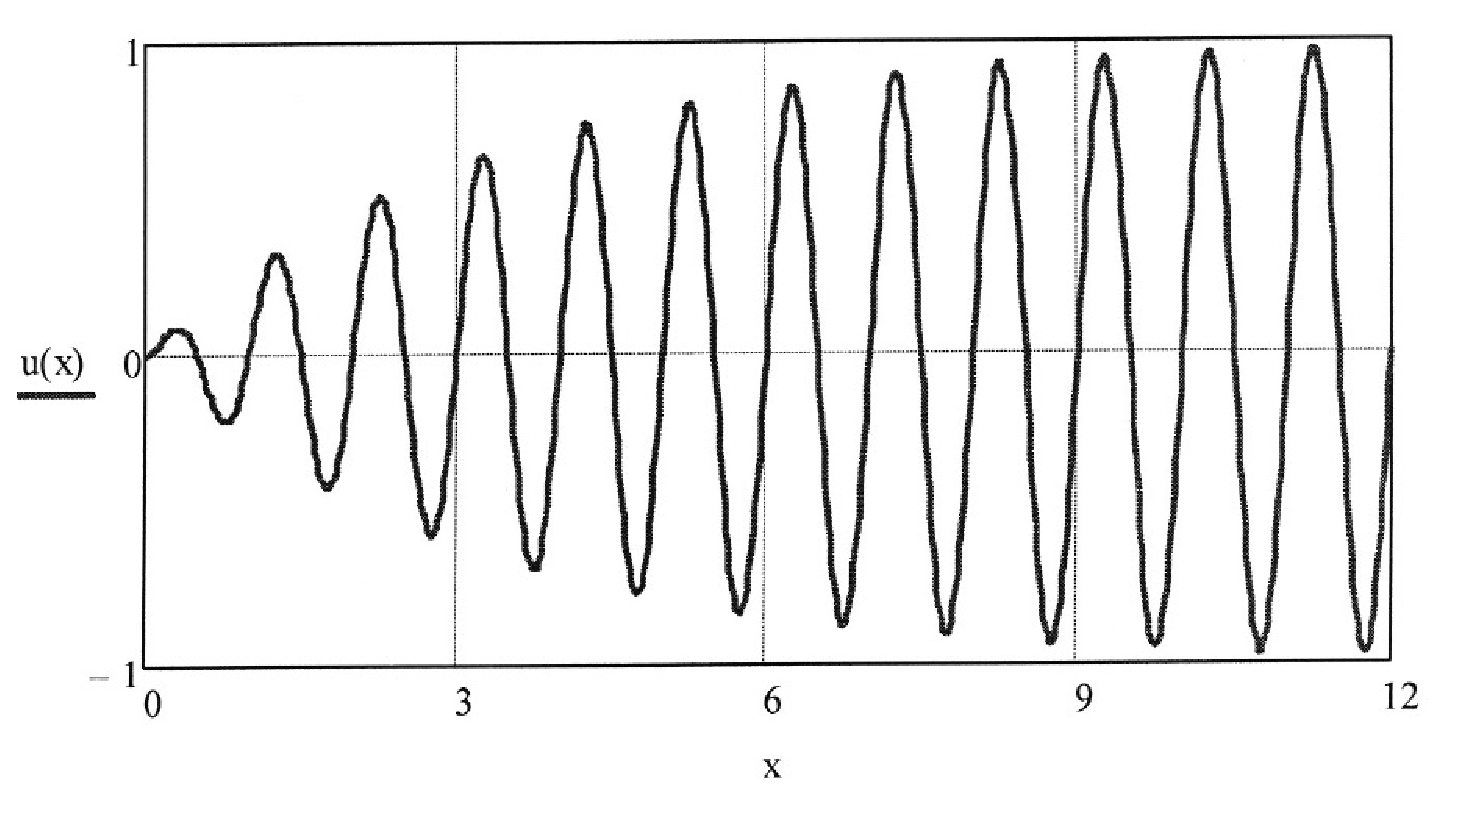
\includegraphics[width=0.6\linewidth]{Chapter_2/13}
    \caption{Волновод и примеры распределения поля} \figmark{waveguide}
\end{figure}

Для бегущих вдоль волновода волн $k_z$~---~действительная величина. Предельный
случай $k_z=0$ соответствует $k=k_x,$ что при условии $n=1$ приводит к формулам
для \important{критических длины и циклической частоты волн}, распространяющихся
в вакуумном волноводе: 
\begin{equation} 
\eqmark{2.0.2} \lambda_{\text{кр}}=2a,
\qquad \omega_{\text{кр}}=\pi c/a. 
\end{equation} 
Если $\lambda>2a$ и,
соответственно, $\omega<\pi c/a,$ то электромагнитная волна при распространении
вдоль волновода затухает.

Для бегущей волны фазовая скорость \begin{equation} \eqmark{2.0.3}
V_{\text{Ф}}=\omega/k_z=c/\sqrt{1-\omega^2_{\text{кр}}/\omega^2} \end{equation}
больше скорости света в вакууме $c,$ а длина волны в волноводе \begin{equation}
\eqmark{2.0.4} \lambda_{\text{В}}=\lambda_0/\sqrt{1-(\lambda_0/2a)^2}
\end{equation} больше длины волны в вакууме $\lambda_0.$ В представленном на
рис.~\figref{waveguide} случае отлична от нуля продольная составляющая
магнитного поля, и такую волну называют \important{магнитной ($H$-волна).}
Обычно для передачи СВЧ-энергии по прямоугольному волноводу используется волна
(мода) $H_{10}.$  Второй индекс $0$ соответствует отсутствию составляющей
электромагнитного поля $E_x.$ Критическая длина волны моды
$H_{10}$~---~максимальная среди всех типов волн в прямоугольном волноводе, и
поэтому ее называют \important{основной.} Тем самым, для волновода заданного
сечения существует диапазон частот, ограниченный снизу критической частотой
волны $H_{10}$ ($\lambda_{\text{кр}}=2a$). Следующая по возрастанию
частоты~---~мода $H_{01}$ с $\lambda_{\text{кр}}=2b$ или $H_{20}$ с
$\lambda_{\text{кр}}=a,$ если $a>b.$

В заданном частотном диапазоне СВЧ-энергия может переноситься одним типом волн,
что существенно облегчает её дальнейшее использование.

Если в волноводе имеется какое-либо препятствие, нерегулярность, то в нём
появляется \important{отражённая волна.} Падающая $E_0$ и отраженная волна с
коэффициентом отражения $\rho$ по амплитуде интерферируют и создают в волноводе
стоячую волну.

Максимальное (в пучности) и минимальное (в узле) значения поля равны
соответственно 
\begin{equation} \eqmark{2.0.5} 
E_{\text{max}}=E_0(1+\rho),
\qquad E_{\text{min}}=E_0(1-\rho). 
\end{equation} 
Отношение
$K=E_{\text{max}}/E_{\text{min}}$ называется \important{коэффициентом стоячей
    волны} (к.с.в.). Коэффициент отражения от препятствия по амплитуде
\begin{equation} \eqmark{2.0.6}
\rho=\dfrac{E_{\text{max}}-E_{\text{min}}}{E_{\text{max}}+E_{\text{min}}}=\dfrac{K-1}{K+1}. 
\end{equation}

В случае полного отражения (металлическая заглушка) $\rho=1,$ а если в волновод
вставлено вещество, поглощающее СВЧ-­излучение (согласованная нагрузка), то
$\rho=0.$

Для определения коэффициента стоячей волны обычно используют измерительную
линию~---~отрезок волновода с продольной щелью длиной в несколько полуволн. В
щели располагается зонд~---~большой металлический штырь (антенна), реагирующий
на электрическое поле в волноводе. Напряжение высокой частоты, наводимое на
зонд, детектируется, усиливается и подаётся на микровольтметр. Зонд может
перемещаться вдоль линии, что позволяет исследовать распределение электрического
поля в волноводе.
